\documentclass[11pt]{article}
\usepackage[textwidth=18.0cm, textheight=23.0cm, top=2.0cm]{geometry}
\usepackage{pst-all}
\usepackage{amssymb}
\usepackage{tikz}
\usepackage{underscore}\begin{document}
\pagestyle{empty}


ClassName: \underline{\textbf{Class_03.2bp-31}}
\par
BinSize: \underline{\textbf{40 × 40}}
\par
ReduceSize: \underline{\textbf{40 × 40}}
\par
TypeNum: \underline{\textbf{76}}
\par
Num: \underline{\textbf{80}}
\par
OutS: \underline{\textbf{28800}}
\par
InS: \underline{\textbf{25445}}
\par
Rate: \underline{\textbf{0.884}}
\par
UB: \underline{\textbf{18}}
\par
LB0: \underline{\textbf{18}}
\par
LB: \underline{\textbf{18}}
\par
LBWithCut: \underline{\textbf{18}}
\par
NodeCut: \underline{\textbf{0}}
\par
ExtendedNodeCnt: \underline{\textbf{1}}
\par
GenNodeCnt: \underline{\textbf{1}}
\par
PrimalNode: \underline{\textbf{0}}
\par
ColumnCount: \underline{\textbf{18}}
\par
TotalCutCount: \underline{\textbf{0}}
\par
RootCutCount: \underline{\textbf{0}}
\par
LPSolverCnt: \underline{\textbf{1}}
\par
PricingSolverCnt: \underline{\textbf{0}}
\par
BranchAndBoundNum: \underline{\textbf{1}}
\par
isOpt: \underline{\textbf{true}}
\par
TimeOnInitSolution: \underline{\textbf{600.000 s}}
\par
TimeOnPrimal: \underline{\textbf{0.000 s}}
\par
TimeOnPricing: \underline{\textbf{0.000 s}}
\par
TimeOnRmp: \underline{\textbf{0.063 s}}
\par
TotalTime: \underline{\textbf{600.329 s}}
\par
\newpage


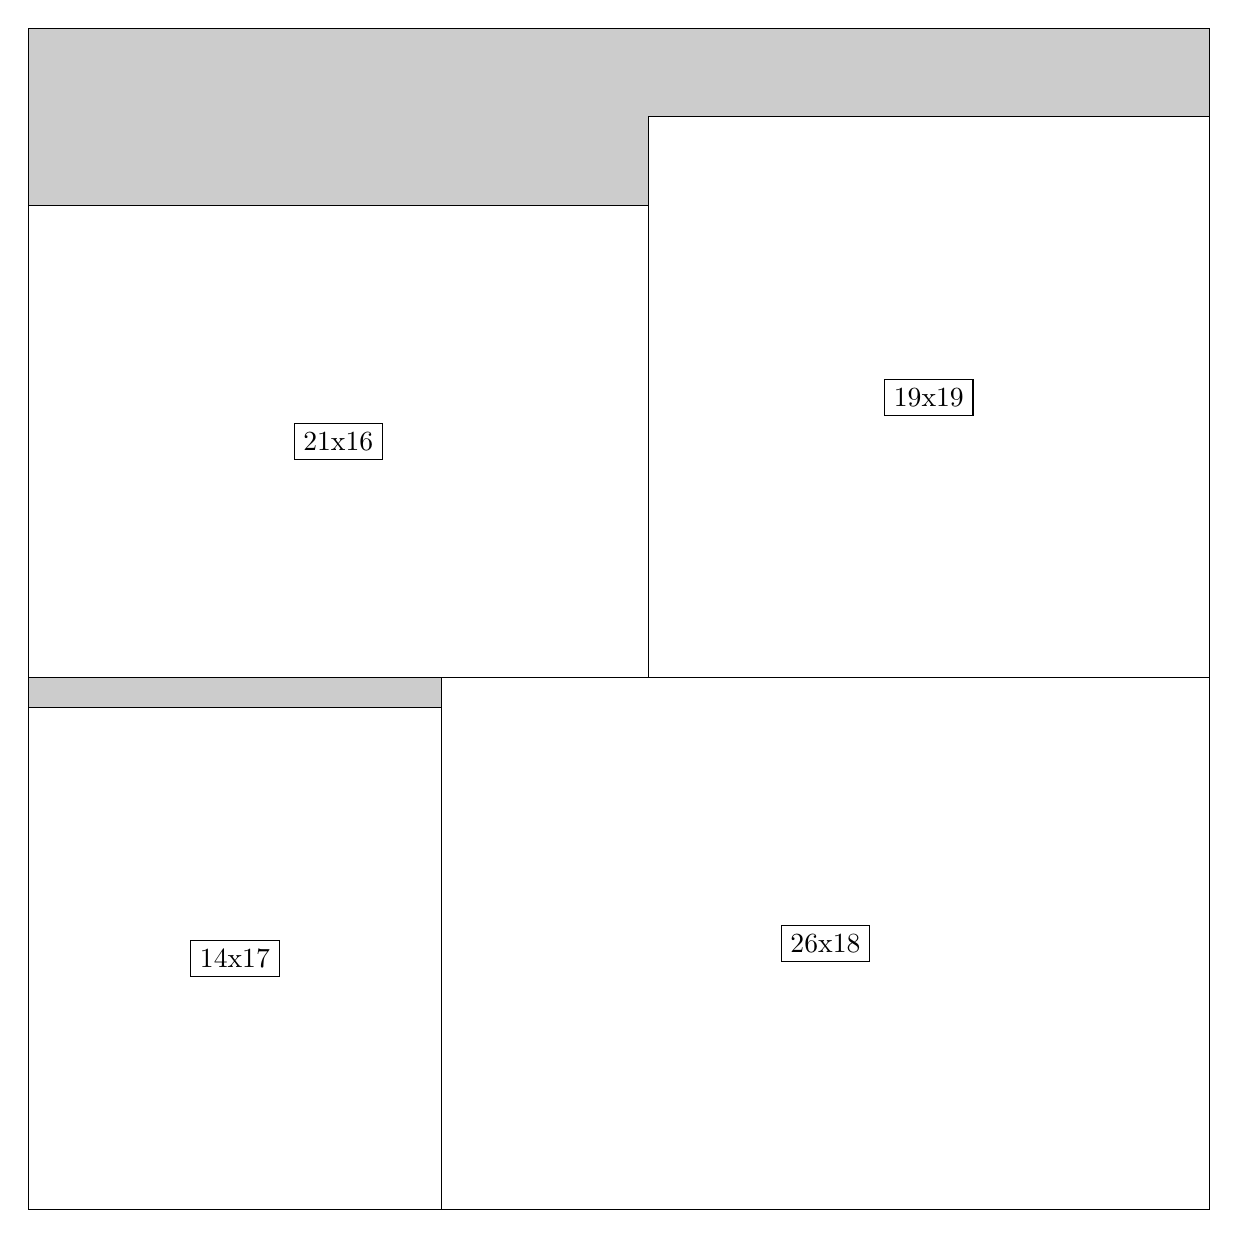
\begin{tikzpicture}[shorten >=1pt,scale=1.0,every node/.style={scale=1.0},->]
\tikzstyle{vertex}=[circle,fill=black!25,minimum size=14pt,inner sep=0pt]
\filldraw[fill=gray!40!white, draw=black] (0,0) rectangle (15.0,15.0);
\foreach \name/\x/\y/\w/\h in {26x18/5.25/0.0/9.75/6.75,14x17/0.0/0.0/5.25/6.375,19x19/7.875/6.75/7.125/7.125,21x16/0.0/6.75/7.875/6.0}
\filldraw[fill=white!40!white, draw=black] (\x,\y) rectangle node[draw] (\name) {\name} ++(\w,\h);
\end{tikzpicture}


w =26 , h =18 , x =14 , y =0 , v =468
\par
w =14 , h =17 , x =0 , y =0 , v =238
\par
w =19 , h =19 , x =21 , y =18 , v =361
\par
w =21 , h =16 , x =0 , y =18 , v =336
\par
\newpage


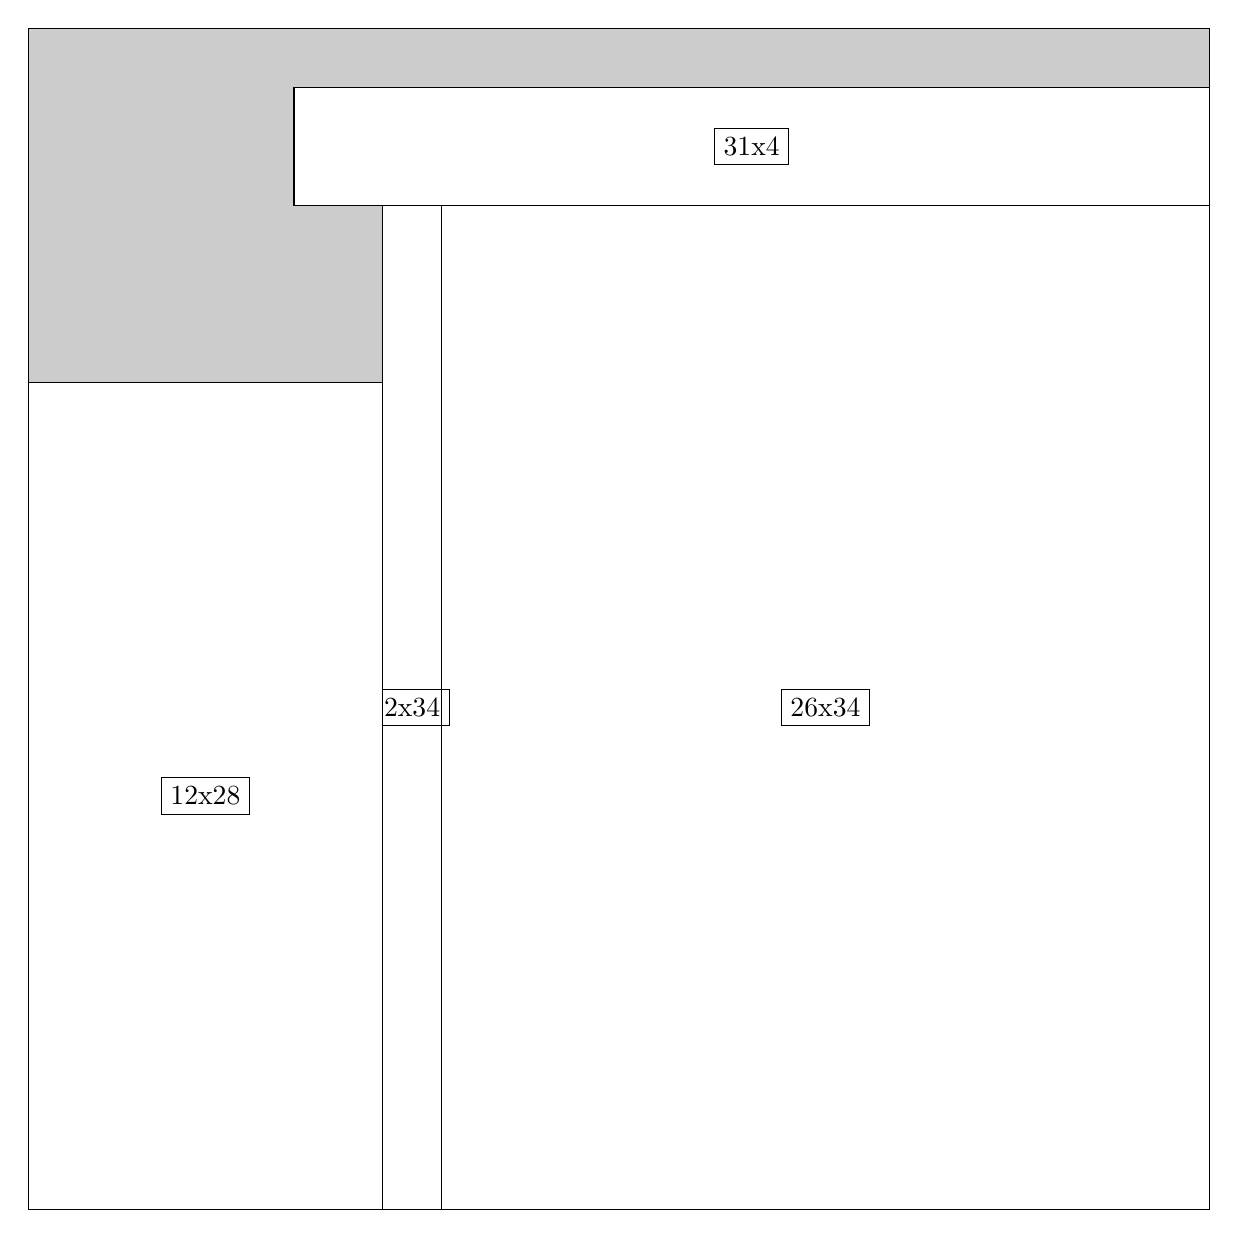
\begin{tikzpicture}[shorten >=1pt,scale=1.0,every node/.style={scale=1.0},->]
\tikzstyle{vertex}=[circle,fill=black!25,minimum size=14pt,inner sep=0pt]
\filldraw[fill=gray!40!white, draw=black] (0,0) rectangle (15.0,15.0);
\foreach \name/\x/\y/\w/\h in {26x34/5.25/0.0/9.75/12.75,2x34/4.5/0.0/0.75/12.75,12x28/0.0/0.0/4.5/10.5,31x4/3.375/12.75/11.625/1.5}
\filldraw[fill=white!40!white, draw=black] (\x,\y) rectangle node[draw] (\name) {\name} ++(\w,\h);
\end{tikzpicture}


w =26 , h =34 , x =14 , y =0 , v =884
\par
w =2 , h =34 , x =12 , y =0 , v =68
\par
w =12 , h =28 , x =0 , y =0 , v =336
\par
w =31 , h =4 , x =9 , y =34 , v =124
\par
\newpage


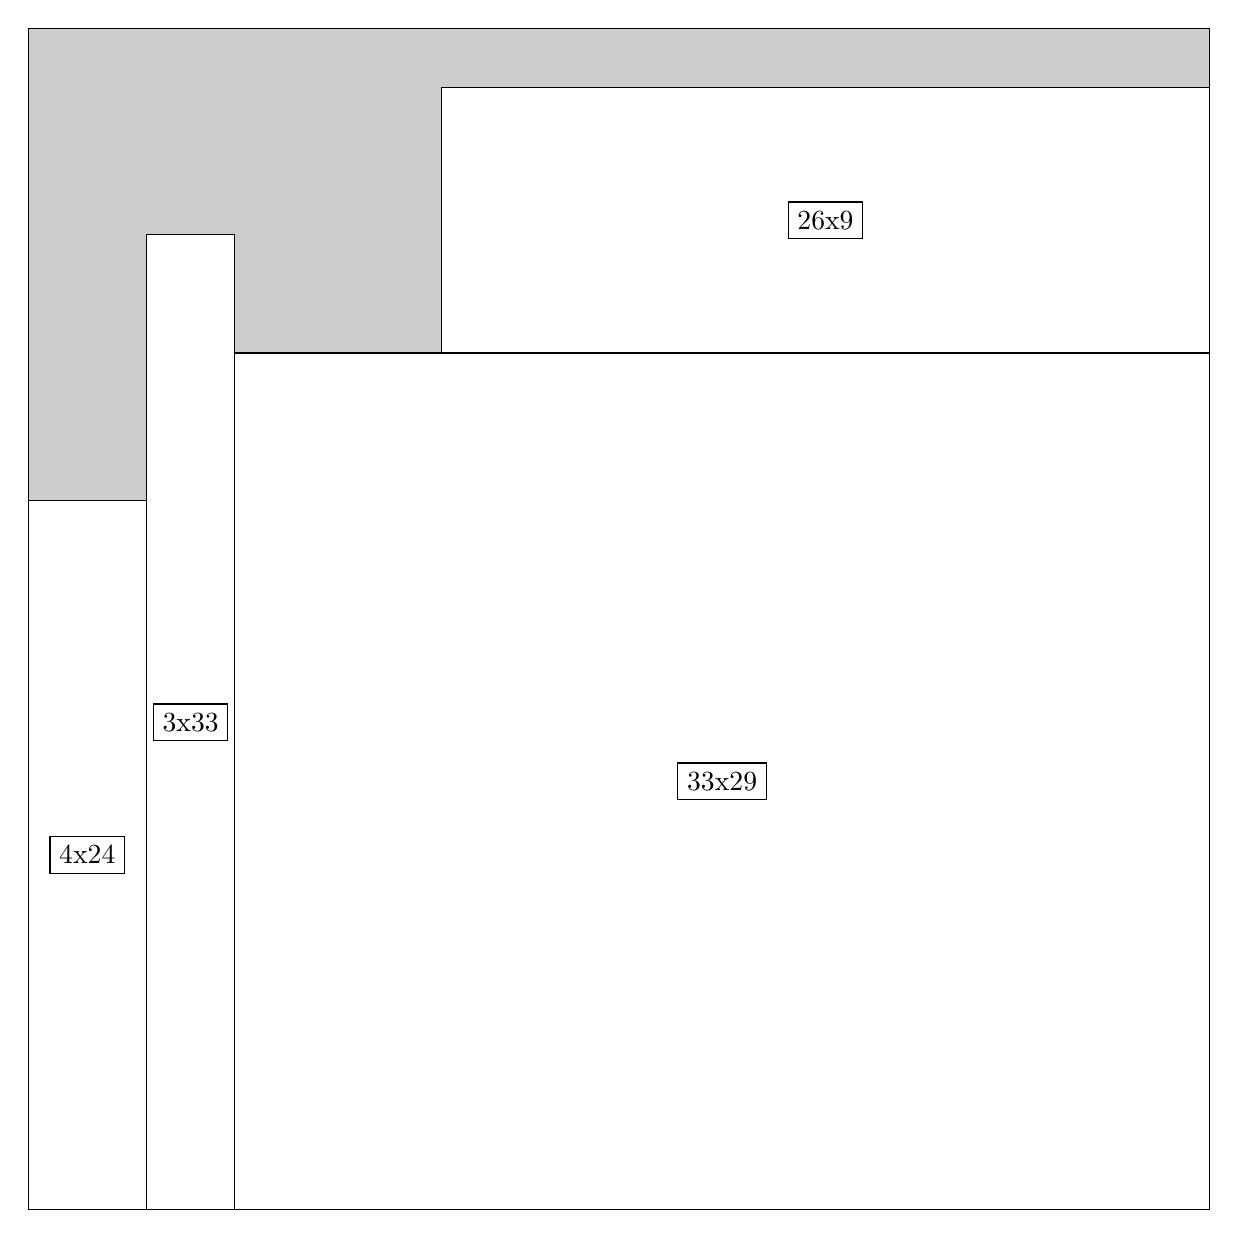
\begin{tikzpicture}[shorten >=1pt,scale=1.0,every node/.style={scale=1.0},->]
\tikzstyle{vertex}=[circle,fill=black!25,minimum size=14pt,inner sep=0pt]
\filldraw[fill=gray!40!white, draw=black] (0,0) rectangle (15.0,15.0);
\foreach \name/\x/\y/\w/\h in {33x29/2.625/0.0/12.375/10.875,26x9/5.25/10.875/9.75/3.375,3x33/1.5/0.0/1.125/12.375,4x24/0.0/0.0/1.5/9.0}
\filldraw[fill=white!40!white, draw=black] (\x,\y) rectangle node[draw] (\name) {\name} ++(\w,\h);
\end{tikzpicture}


w =33 , h =29 , x =7 , y =0 , v =957
\par
w =26 , h =9 , x =14 , y =29 , v =234
\par
w =3 , h =33 , x =4 , y =0 , v =99
\par
w =4 , h =24 , x =0 , y =0 , v =96
\par
\newpage


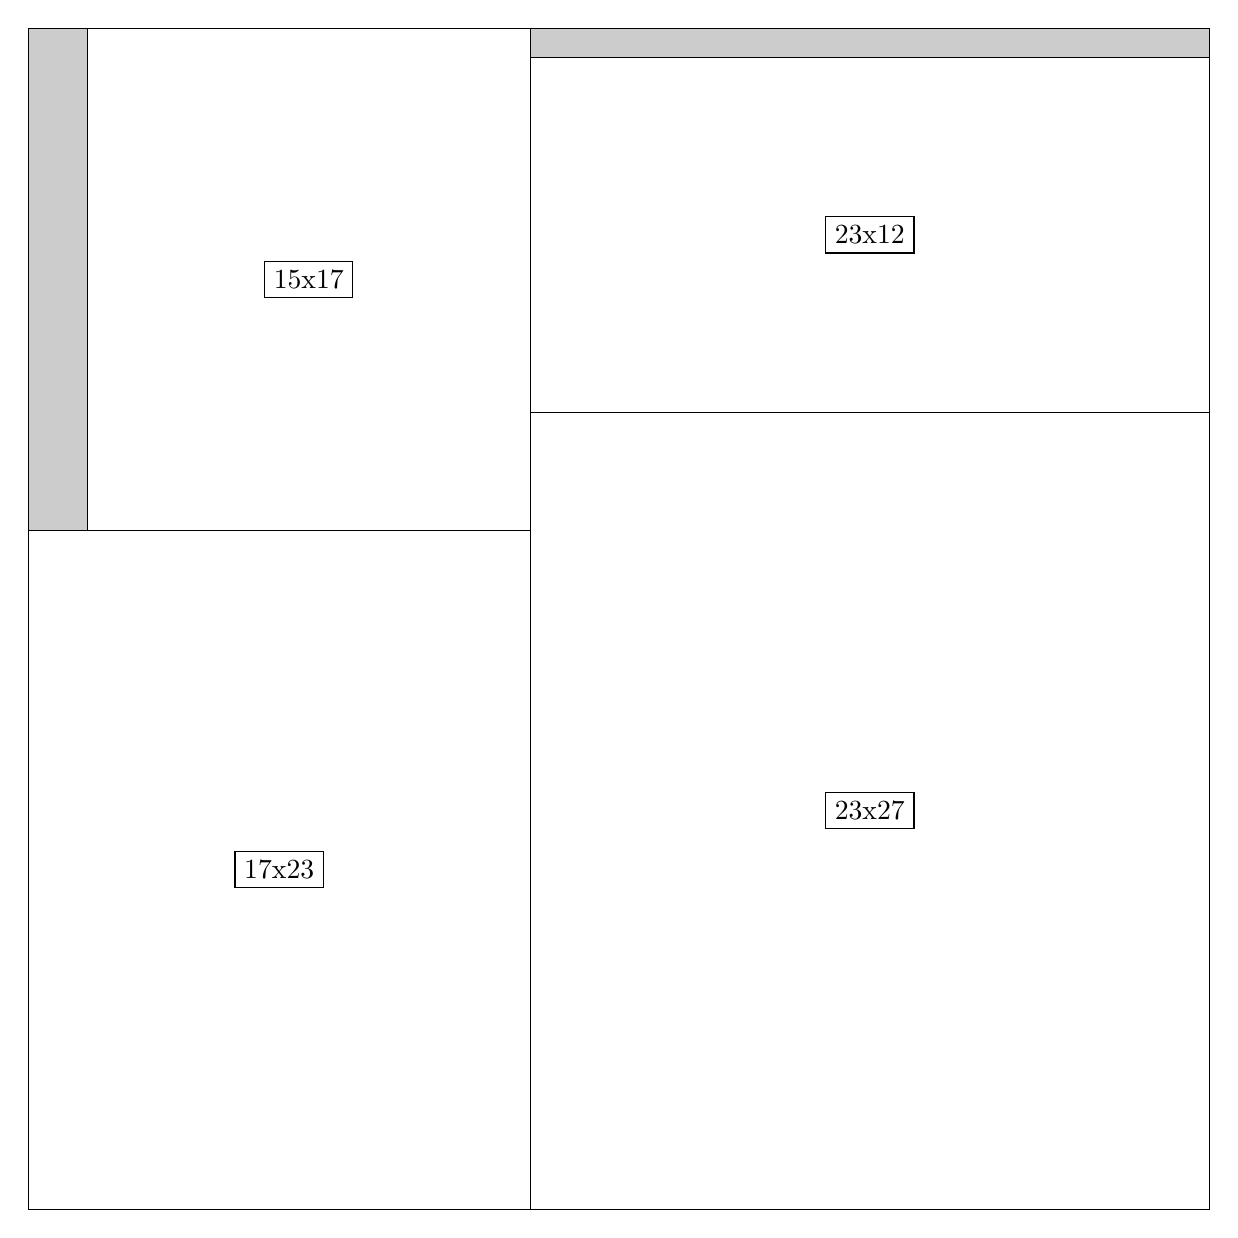
\begin{tikzpicture}[shorten >=1pt,scale=1.0,every node/.style={scale=1.0},->]
\tikzstyle{vertex}=[circle,fill=black!25,minimum size=14pt,inner sep=0pt]
\filldraw[fill=gray!40!white, draw=black] (0,0) rectangle (15.0,15.0);
\foreach \name/\x/\y/\w/\h in {23x27/6.375/0.0/8.625/10.125,23x12/6.375/10.125/8.625/4.5,17x23/0.0/0.0/6.375/8.625,15x17/0.75/8.625/5.625/6.375}
\filldraw[fill=white!40!white, draw=black] (\x,\y) rectangle node[draw] (\name) {\name} ++(\w,\h);
\end{tikzpicture}


w =23 , h =27 , x =17 , y =0 , v =621
\par
w =23 , h =12 , x =17 , y =27 , v =276
\par
w =17 , h =23 , x =0 , y =0 , v =391
\par
w =15 , h =17 , x =2 , y =23 , v =255
\par
\newpage


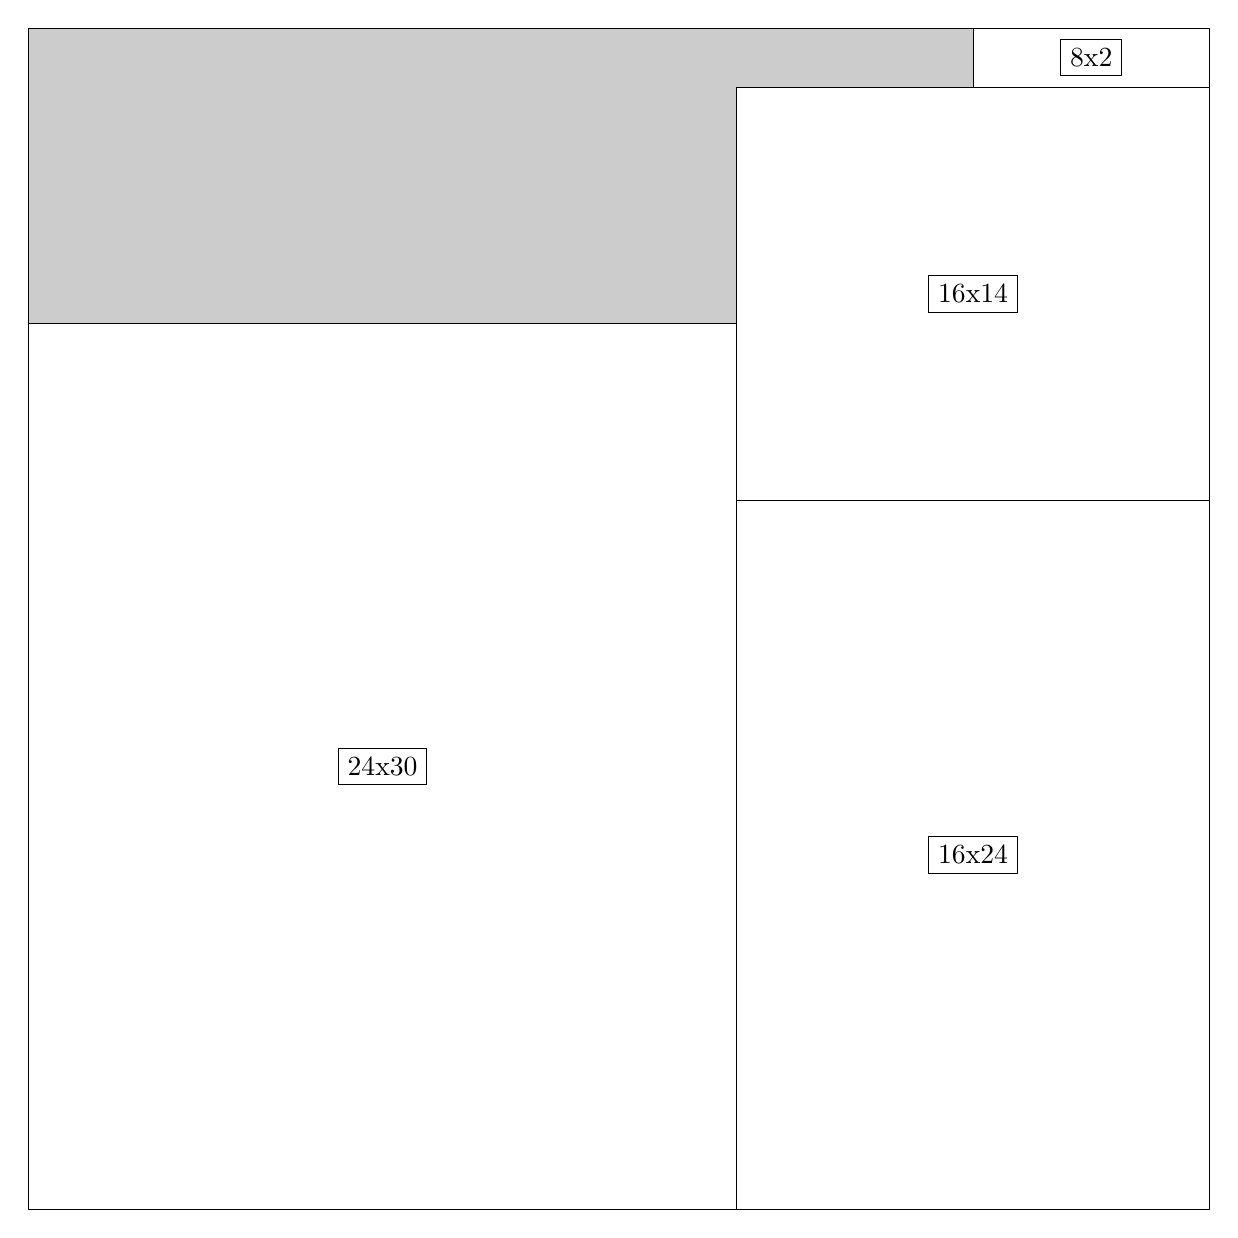
\begin{tikzpicture}[shorten >=1pt,scale=1.0,every node/.style={scale=1.0},->]
\tikzstyle{vertex}=[circle,fill=black!25,minimum size=14pt,inner sep=0pt]
\filldraw[fill=gray!40!white, draw=black] (0,0) rectangle (15.0,15.0);
\foreach \name/\x/\y/\w/\h in {16x24/9.0/0.0/6.0/9.0,16x14/9.0/9.0/6.0/5.25,8x2/12.0/14.25/3.0/0.75,24x30/0.0/0.0/9.0/11.25}
\filldraw[fill=white!40!white, draw=black] (\x,\y) rectangle node[draw] (\name) {\name} ++(\w,\h);
\end{tikzpicture}


w =16 , h =24 , x =24 , y =0 , v =384
\par
w =16 , h =14 , x =24 , y =24 , v =224
\par
w =8 , h =2 , x =32 , y =38 , v =16
\par
w =24 , h =30 , x =0 , y =0 , v =720
\par
\newpage


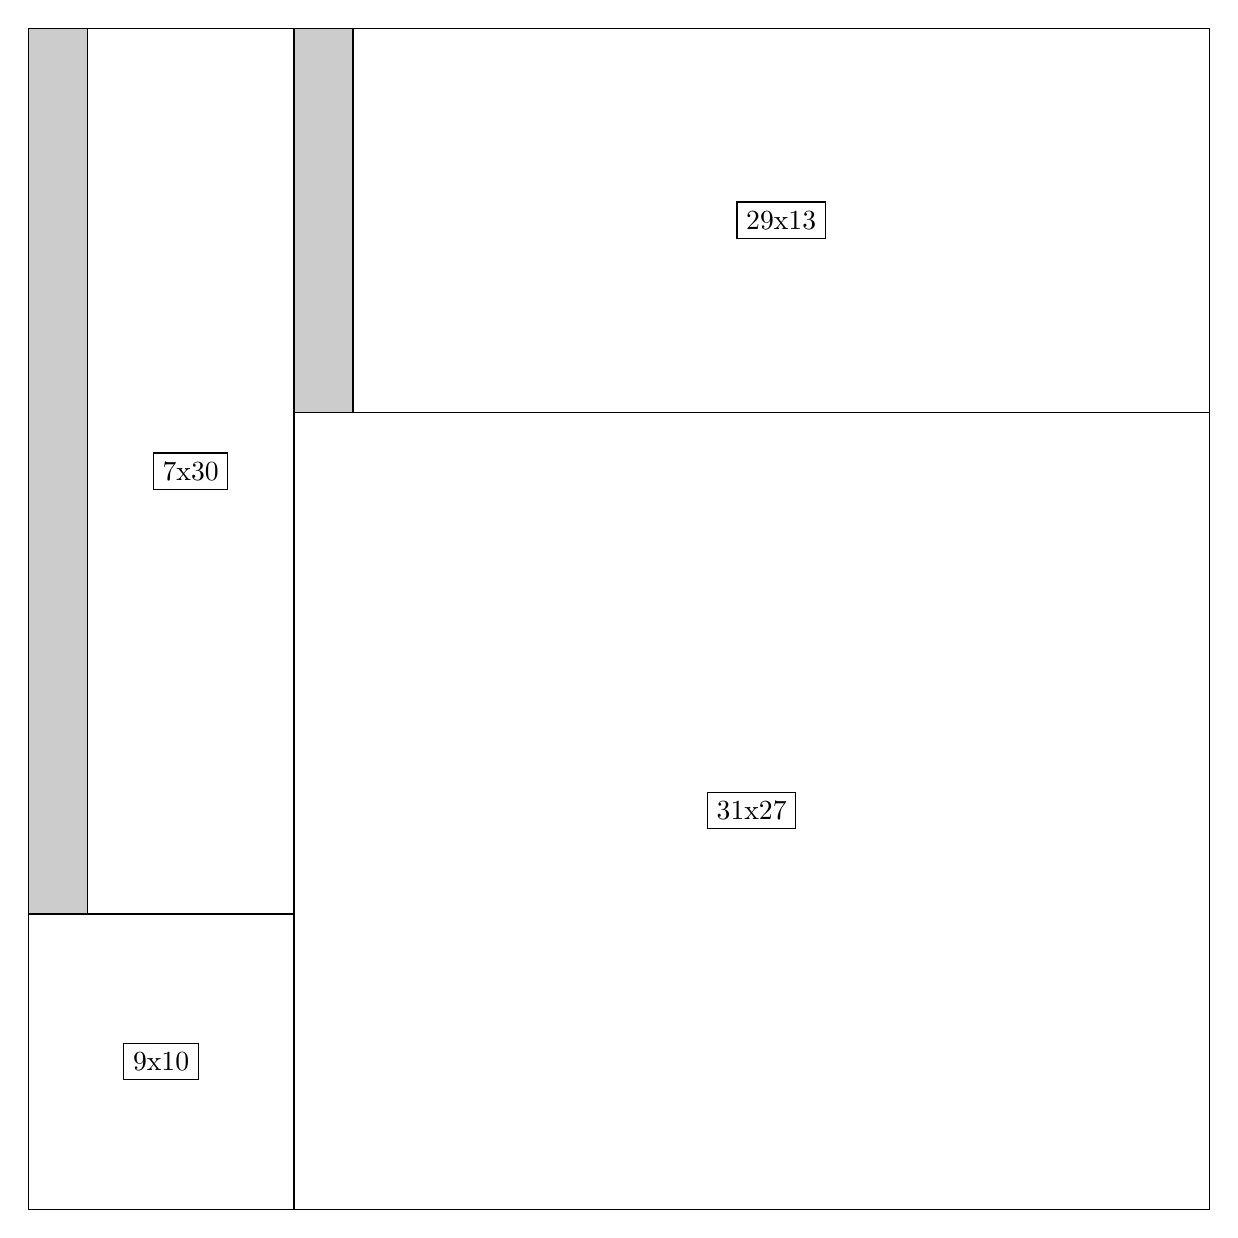
\begin{tikzpicture}[shorten >=1pt,scale=1.0,every node/.style={scale=1.0},->]
\tikzstyle{vertex}=[circle,fill=black!25,minimum size=14pt,inner sep=0pt]
\filldraw[fill=gray!40!white, draw=black] (0,0) rectangle (15.0,15.0);
\foreach \name/\x/\y/\w/\h in {31x27/3.375/0.0/11.625/10.125,29x13/4.125/10.125/10.875/4.875,9x10/0.0/0.0/3.375/3.75,7x30/0.75/3.75/2.625/11.25}
\filldraw[fill=white!40!white, draw=black] (\x,\y) rectangle node[draw] (\name) {\name} ++(\w,\h);
\end{tikzpicture}


w =31 , h =27 , x =9 , y =0 , v =837
\par
w =29 , h =13 , x =11 , y =27 , v =377
\par
w =9 , h =10 , x =0 , y =0 , v =90
\par
w =7 , h =30 , x =2 , y =10 , v =210
\par
\newpage


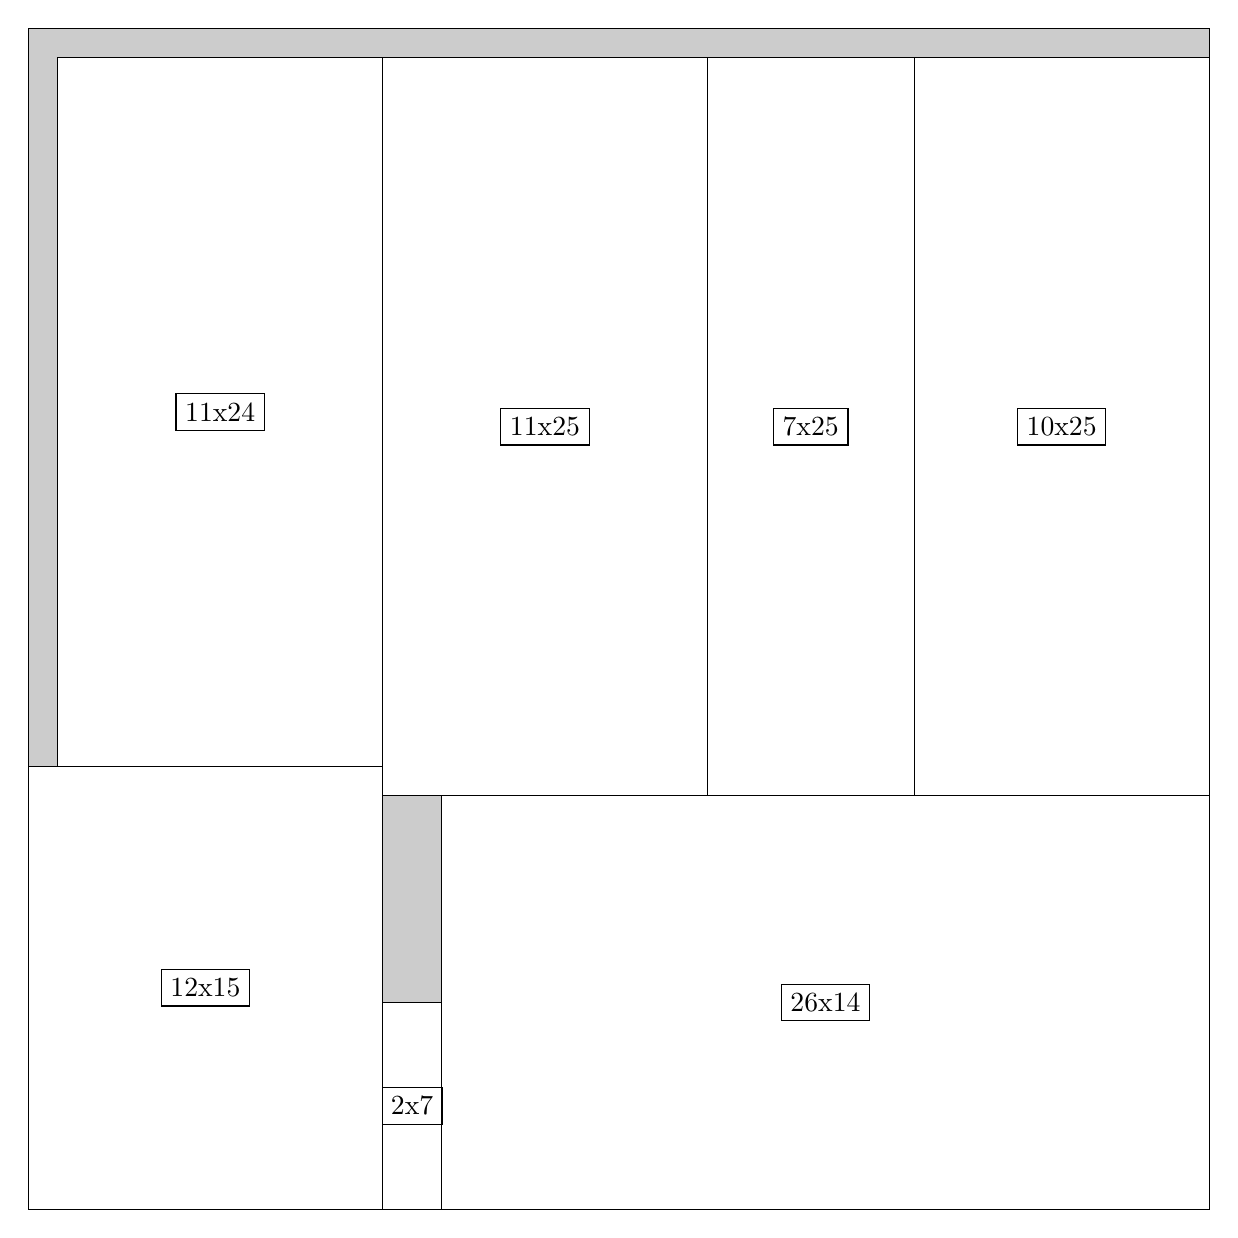
\begin{tikzpicture}[shorten >=1pt,scale=1.0,every node/.style={scale=1.0},->]
\tikzstyle{vertex}=[circle,fill=black!25,minimum size=14pt,inner sep=0pt]
\filldraw[fill=gray!40!white, draw=black] (0,0) rectangle (15.0,15.0);
\foreach \name/\x/\y/\w/\h in {26x14/5.25/0.0/9.75/5.25,2x7/4.5/0.0/0.75/2.625,10x25/11.25/5.25/3.75/9.375,7x25/8.625/5.25/2.625/9.375,11x25/4.5/5.25/4.125/9.375,12x15/0.0/0.0/4.5/5.625,11x24/0.375/5.625/4.125/9.0}
\filldraw[fill=white!40!white, draw=black] (\x,\y) rectangle node[draw] (\name) {\name} ++(\w,\h);
\end{tikzpicture}


w =26 , h =14 , x =14 , y =0 , v =364
\par
w =2 , h =7 , x =12 , y =0 , v =14
\par
w =10 , h =25 , x =30 , y =14 , v =250
\par
w =7 , h =25 , x =23 , y =14 , v =175
\par
w =11 , h =25 , x =12 , y =14 , v =275
\par
w =12 , h =15 , x =0 , y =0 , v =180
\par
w =11 , h =24 , x =1 , y =15 , v =264
\par
\newpage


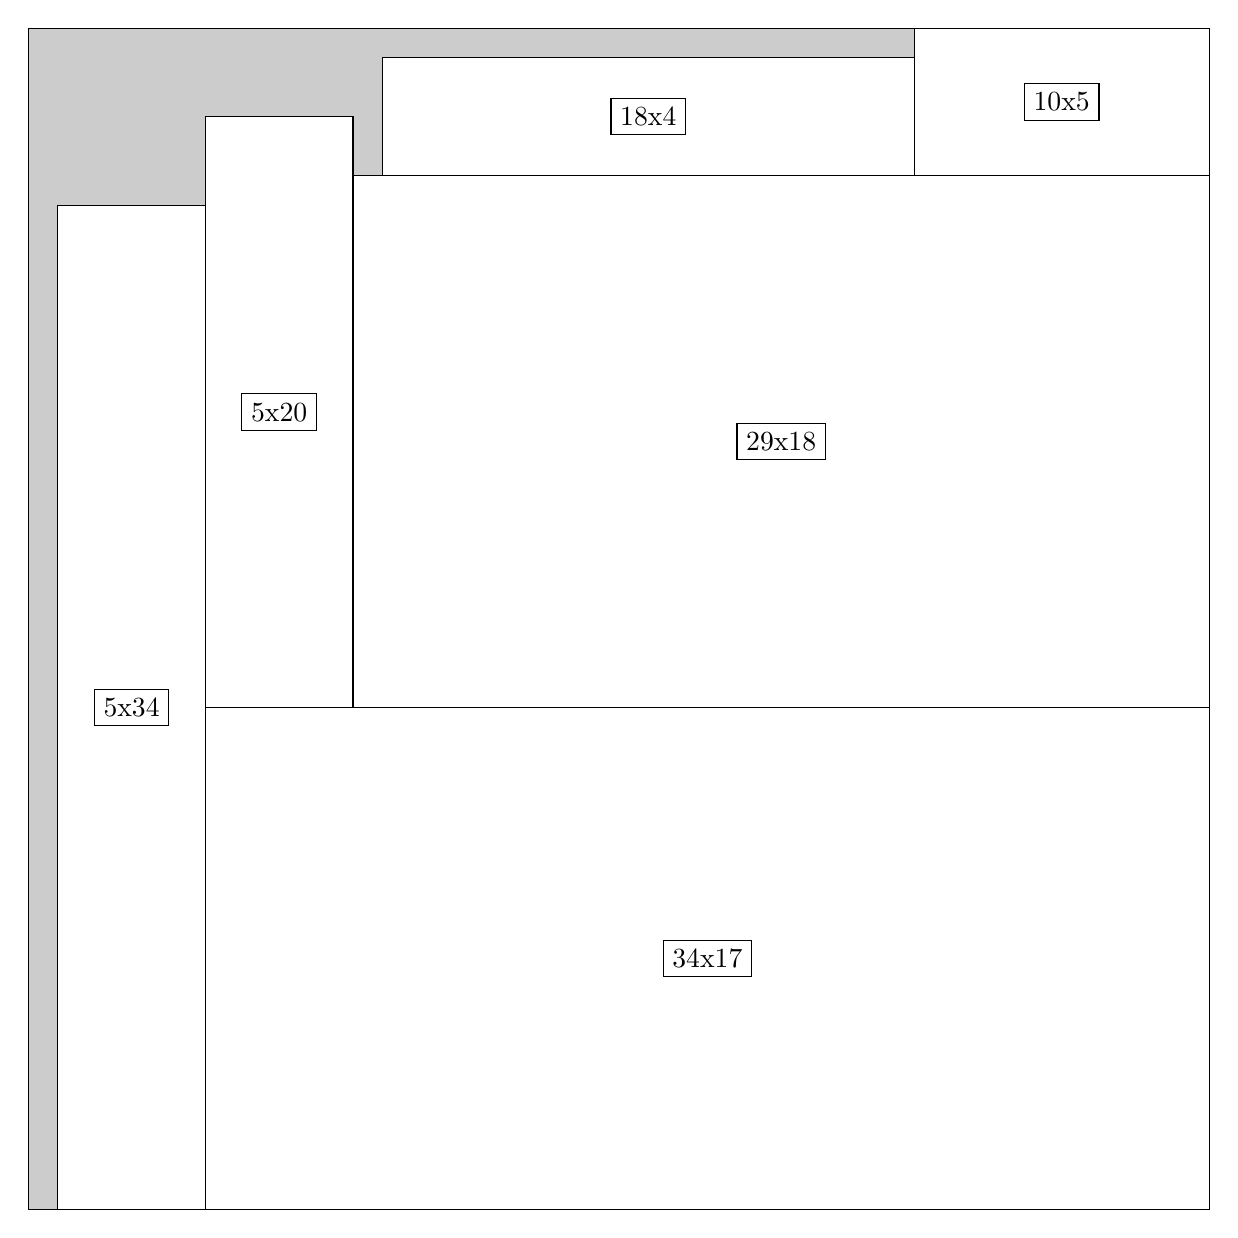
\begin{tikzpicture}[shorten >=1pt,scale=1.0,every node/.style={scale=1.0},->]
\tikzstyle{vertex}=[circle,fill=black!25,minimum size=14pt,inner sep=0pt]
\filldraw[fill=gray!40!white, draw=black] (0,0) rectangle (15.0,15.0);
\foreach \name/\x/\y/\w/\h in {34x17/2.25/0.0/12.75/6.375,29x18/4.125/6.375/10.875/6.75,10x5/11.25/13.125/3.75/1.875,18x4/4.5/13.125/6.75/1.5,5x20/2.25/6.375/1.875/7.5,5x34/0.375/0.0/1.875/12.75}
\filldraw[fill=white!40!white, draw=black] (\x,\y) rectangle node[draw] (\name) {\name} ++(\w,\h);
\end{tikzpicture}


w =34 , h =17 , x =6 , y =0 , v =578
\par
w =29 , h =18 , x =11 , y =17 , v =522
\par
w =10 , h =5 , x =30 , y =35 , v =50
\par
w =18 , h =4 , x =12 , y =35 , v =72
\par
w =5 , h =20 , x =6 , y =17 , v =100
\par
w =5 , h =34 , x =1 , y =0 , v =170
\par
\newpage


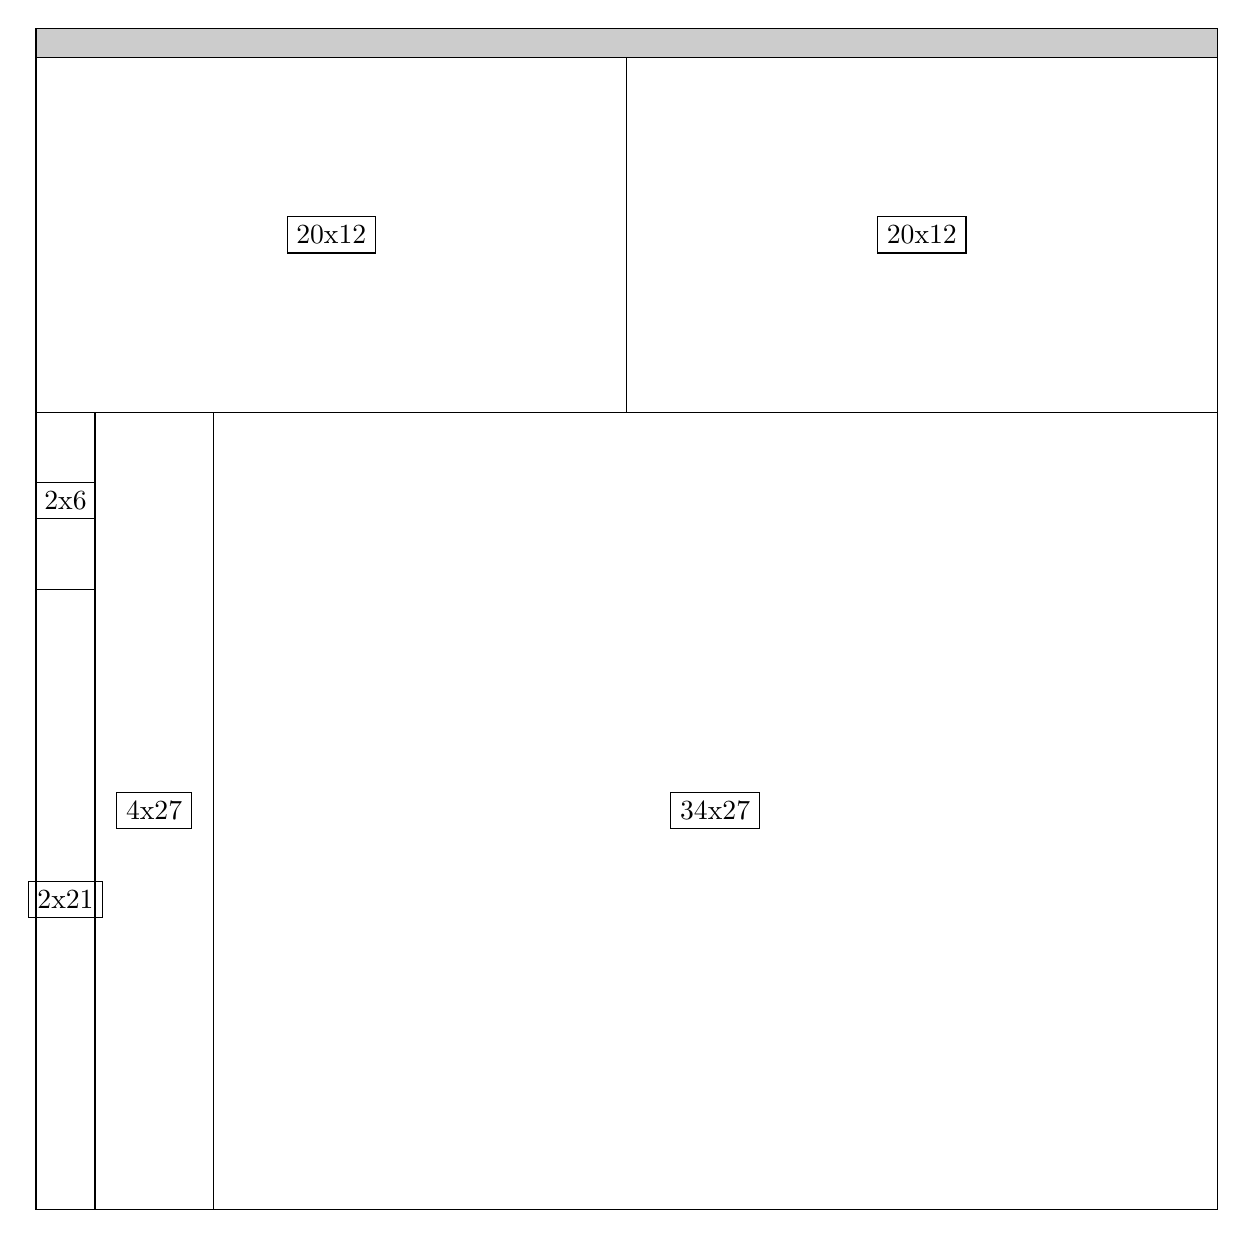
\begin{tikzpicture}[shorten >=1pt,scale=1.0,every node/.style={scale=1.0},->]
\tikzstyle{vertex}=[circle,fill=black!25,minimum size=14pt,inner sep=0pt]
\filldraw[fill=gray!40!white, draw=black] (0,0) rectangle (15.0,15.0);
\foreach \name/\x/\y/\w/\h in {34x27/2.25/0.0/12.75/10.125,4x27/0.75/0.0/1.5/10.125,2x21/0.0/0.0/0.75/7.875,2x6/0.0/7.875/0.75/2.25,20x12/7.5/10.125/7.5/4.5,20x12/0.0/10.125/7.5/4.5}
\filldraw[fill=white!40!white, draw=black] (\x,\y) rectangle node[draw] (\name) {\name} ++(\w,\h);
\end{tikzpicture}


w =34 , h =27 , x =6 , y =0 , v =918
\par
w =4 , h =27 , x =2 , y =0 , v =108
\par
w =2 , h =21 , x =0 , y =0 , v =42
\par
w =2 , h =6 , x =0 , y =21 , v =12
\par
w =20 , h =12 , x =20 , y =27 , v =240
\par
w =20 , h =12 , x =0 , y =27 , v =240
\par
\newpage


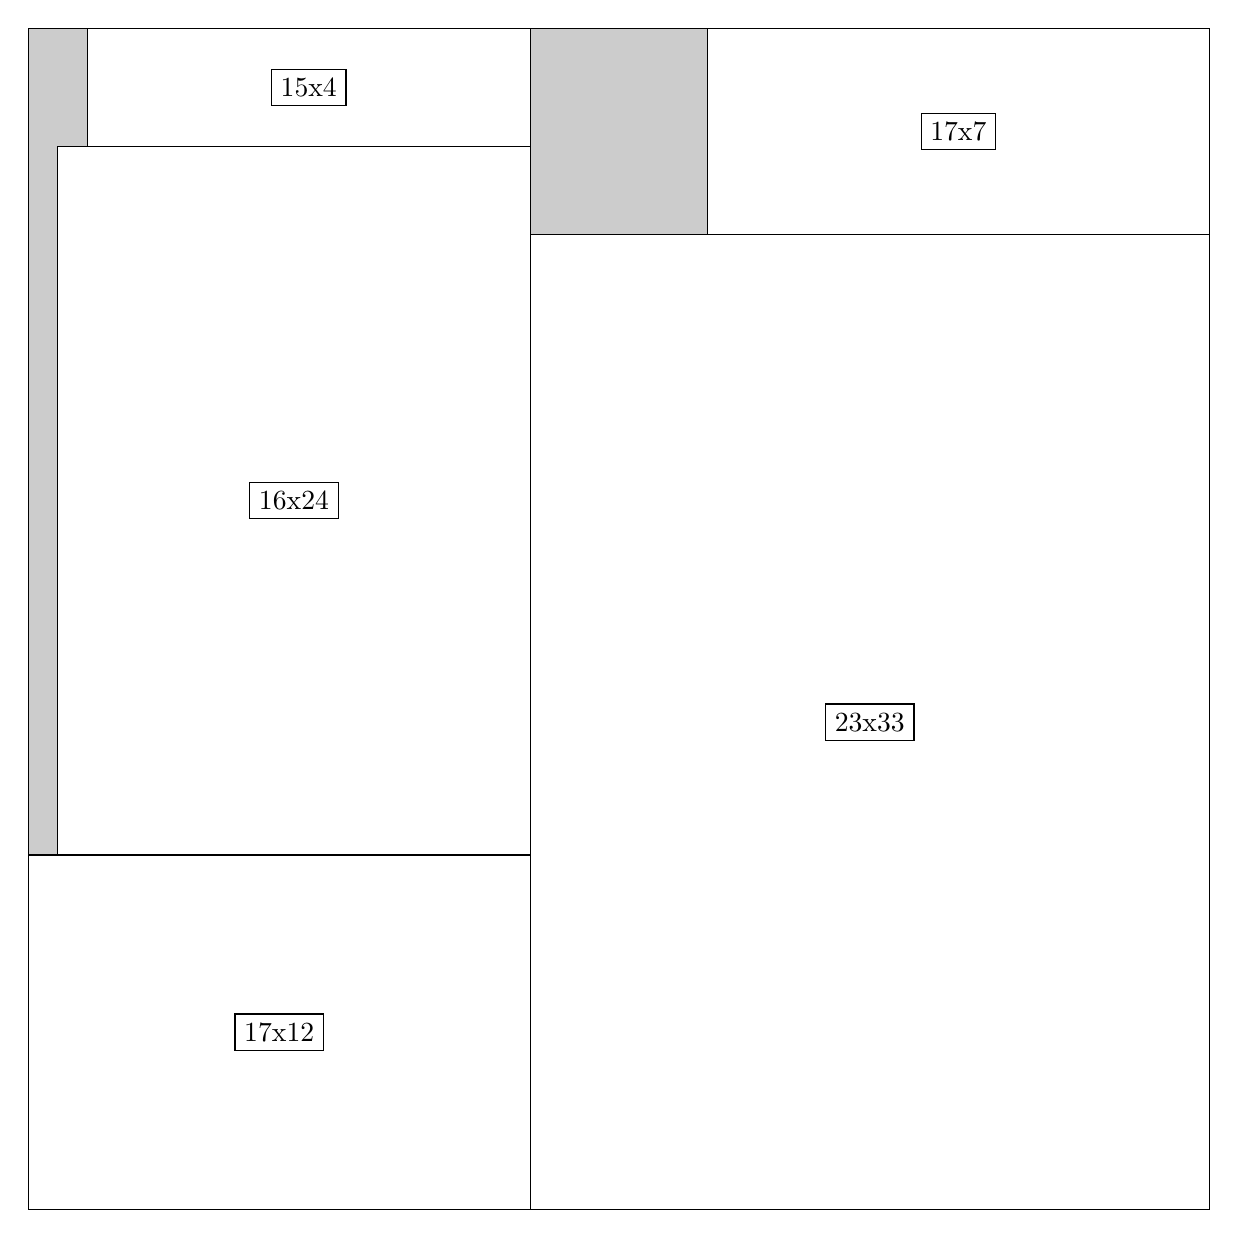
\begin{tikzpicture}[shorten >=1pt,scale=1.0,every node/.style={scale=1.0},->]
\tikzstyle{vertex}=[circle,fill=black!25,minimum size=14pt,inner sep=0pt]
\filldraw[fill=gray!40!white, draw=black] (0,0) rectangle (15.0,15.0);
\foreach \name/\x/\y/\w/\h in {23x33/6.375/0.0/8.625/12.375,17x7/8.625/12.375/6.375/2.625,17x12/0.0/0.0/6.375/4.5,16x24/0.375/4.5/6.0/9.0,15x4/0.75/13.5/5.625/1.5}
\filldraw[fill=white!40!white, draw=black] (\x,\y) rectangle node[draw] (\name) {\name} ++(\w,\h);
\end{tikzpicture}


w =23 , h =33 , x =17 , y =0 , v =759
\par
w =17 , h =7 , x =23 , y =33 , v =119
\par
w =17 , h =12 , x =0 , y =0 , v =204
\par
w =16 , h =24 , x =1 , y =12 , v =384
\par
w =15 , h =4 , x =2 , y =36 , v =60
\par
\newpage


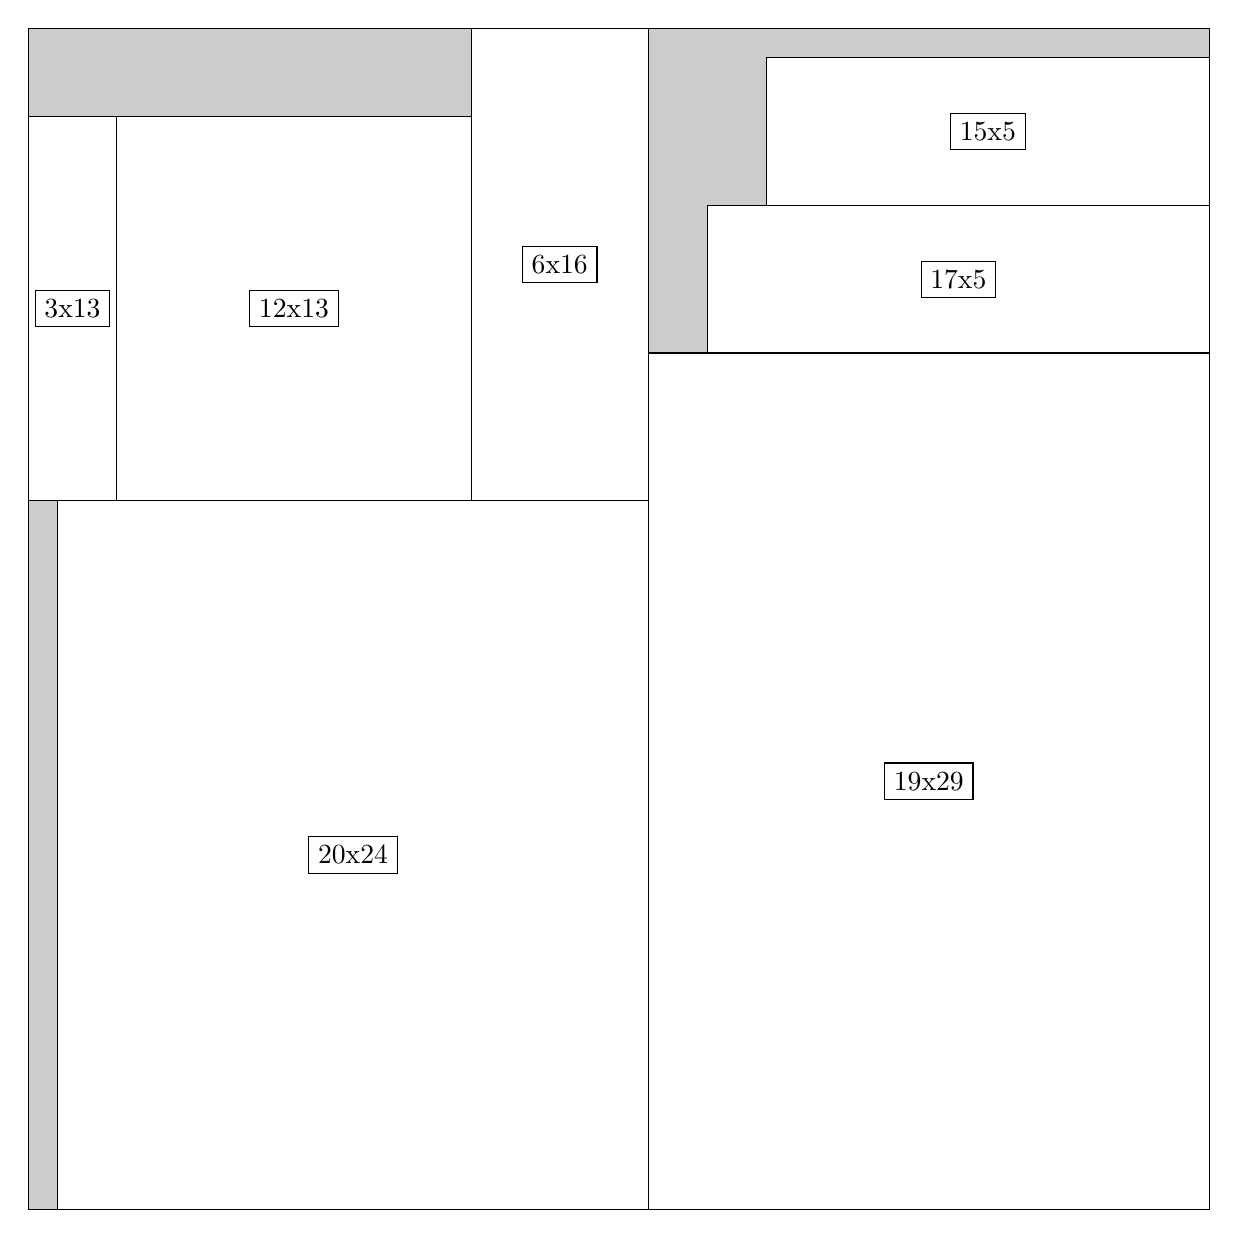
\begin{tikzpicture}[shorten >=1pt,scale=1.0,every node/.style={scale=1.0},->]
\tikzstyle{vertex}=[circle,fill=black!25,minimum size=14pt,inner sep=0pt]
\filldraw[fill=gray!40!white, draw=black] (0,0) rectangle (15.0,15.0);
\foreach \name/\x/\y/\w/\h in {19x29/7.875/0.0/7.125/10.875,17x5/8.625/10.875/6.375/1.875,15x5/9.375/12.75/5.625/1.875,20x24/0.375/0.0/7.5/9.0,6x16/5.625/9.0/2.25/6.0,12x13/1.125/9.0/4.5/4.875,3x13/0.0/9.0/1.125/4.875}
\filldraw[fill=white!40!white, draw=black] (\x,\y) rectangle node[draw] (\name) {\name} ++(\w,\h);
\end{tikzpicture}


w =19 , h =29 , x =21 , y =0 , v =551
\par
w =17 , h =5 , x =23 , y =29 , v =85
\par
w =15 , h =5 , x =25 , y =34 , v =75
\par
w =20 , h =24 , x =1 , y =0 , v =480
\par
w =6 , h =16 , x =15 , y =24 , v =96
\par
w =12 , h =13 , x =3 , y =24 , v =156
\par
w =3 , h =13 , x =0 , y =24 , v =39
\par
\newpage


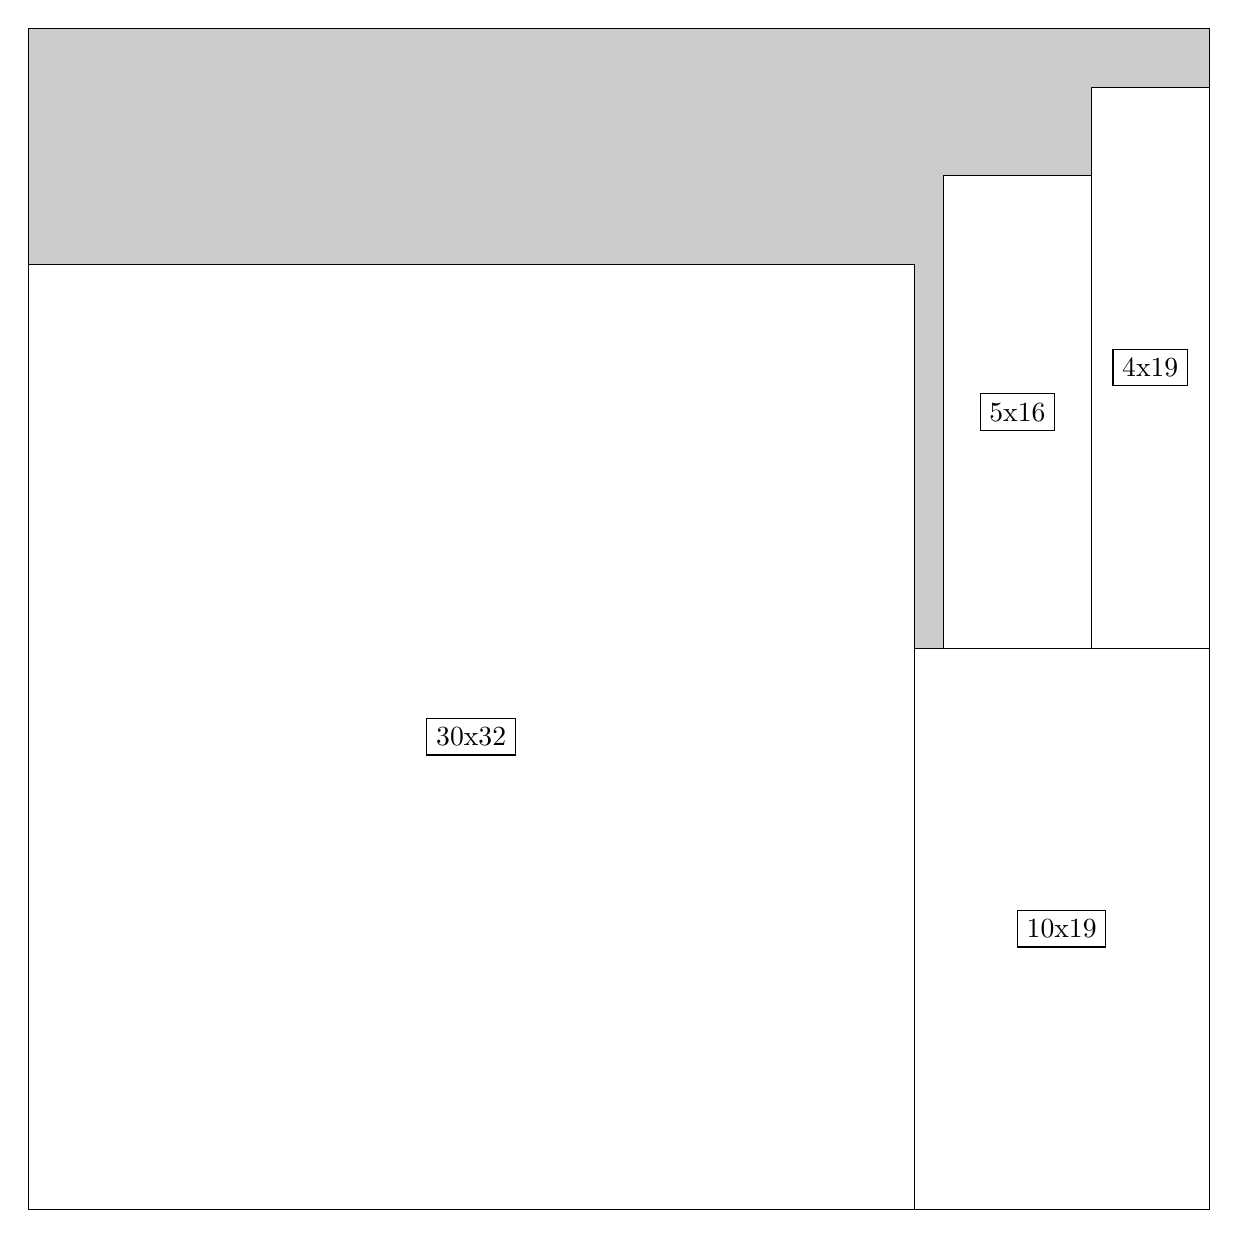
\begin{tikzpicture}[shorten >=1pt,scale=1.0,every node/.style={scale=1.0},->]
\tikzstyle{vertex}=[circle,fill=black!25,minimum size=14pt,inner sep=0pt]
\filldraw[fill=gray!40!white, draw=black] (0,0) rectangle (15.0,15.0);
\foreach \name/\x/\y/\w/\h in {10x19/11.25/0.0/3.75/7.125,4x19/13.5/7.125/1.5/7.125,5x16/11.625/7.125/1.875/6.0,30x32/0.0/0.0/11.25/12.0}
\filldraw[fill=white!40!white, draw=black] (\x,\y) rectangle node[draw] (\name) {\name} ++(\w,\h);
\end{tikzpicture}


w =10 , h =19 , x =30 , y =0 , v =190
\par
w =4 , h =19 , x =36 , y =19 , v =76
\par
w =5 , h =16 , x =31 , y =19 , v =80
\par
w =30 , h =32 , x =0 , y =0 , v =960
\par
\newpage


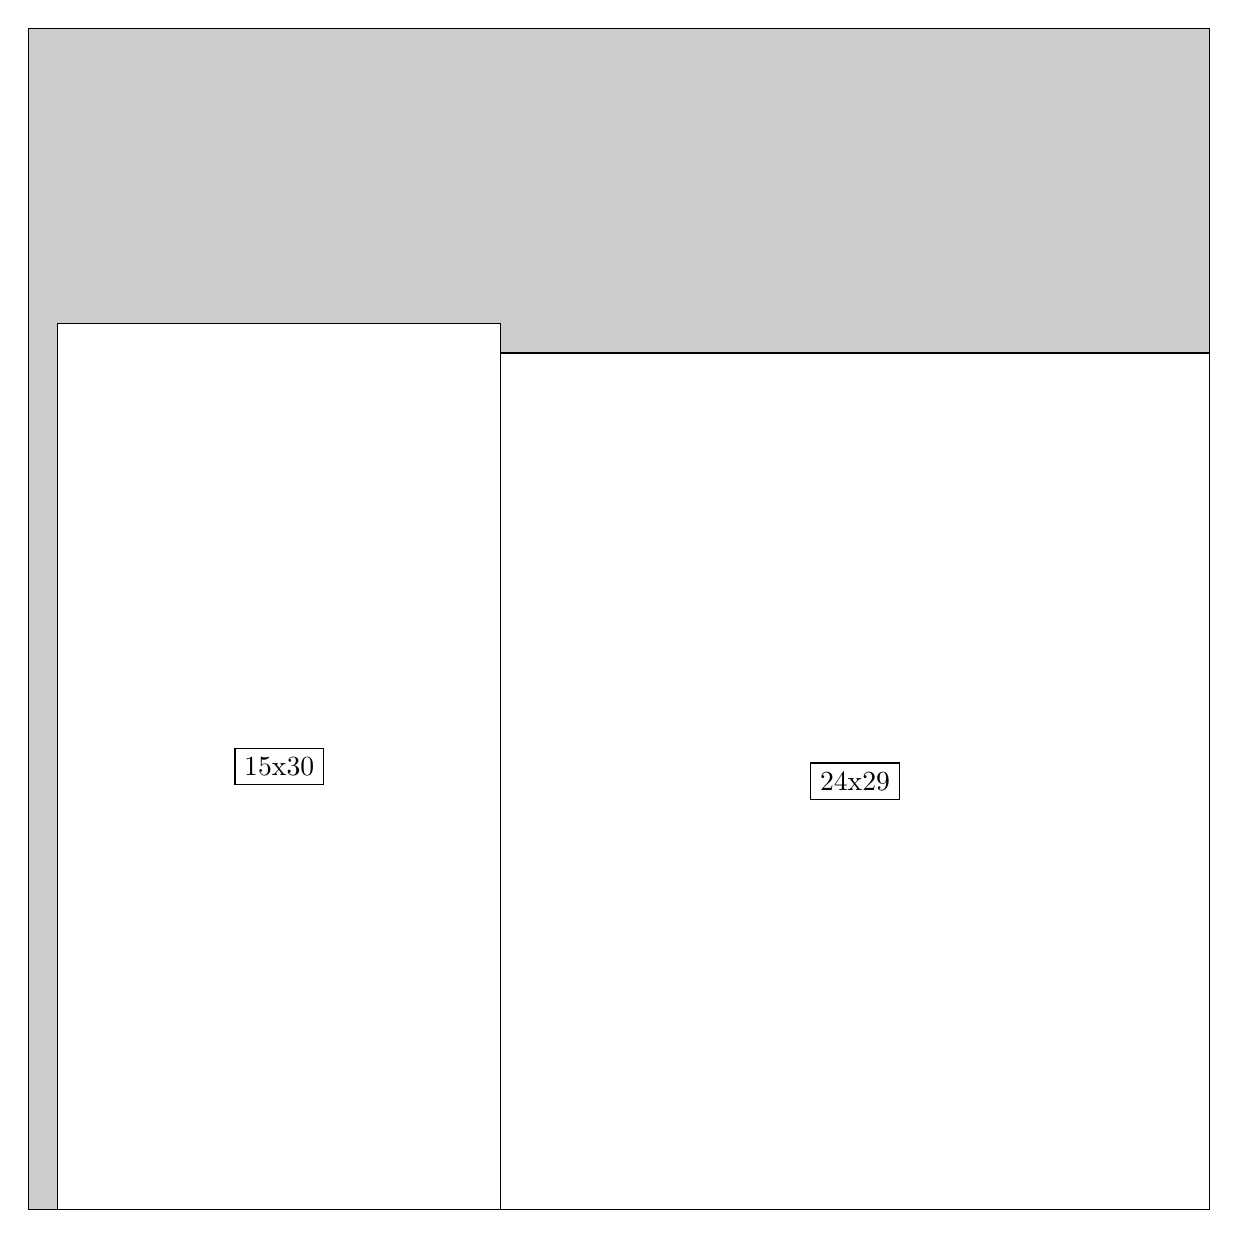
\begin{tikzpicture}[shorten >=1pt,scale=1.0,every node/.style={scale=1.0},->]
\tikzstyle{vertex}=[circle,fill=black!25,minimum size=14pt,inner sep=0pt]
\filldraw[fill=gray!40!white, draw=black] (0,0) rectangle (15.0,15.0);
\foreach \name/\x/\y/\w/\h in {24x29/6.0/0.0/9.0/10.875,15x30/0.375/0.0/5.625/11.25}
\filldraw[fill=white!40!white, draw=black] (\x,\y) rectangle node[draw] (\name) {\name} ++(\w,\h);
\end{tikzpicture}


w =24 , h =29 , x =16 , y =0 , v =696
\par
w =15 , h =30 , x =1 , y =0 , v =450
\par
\newpage


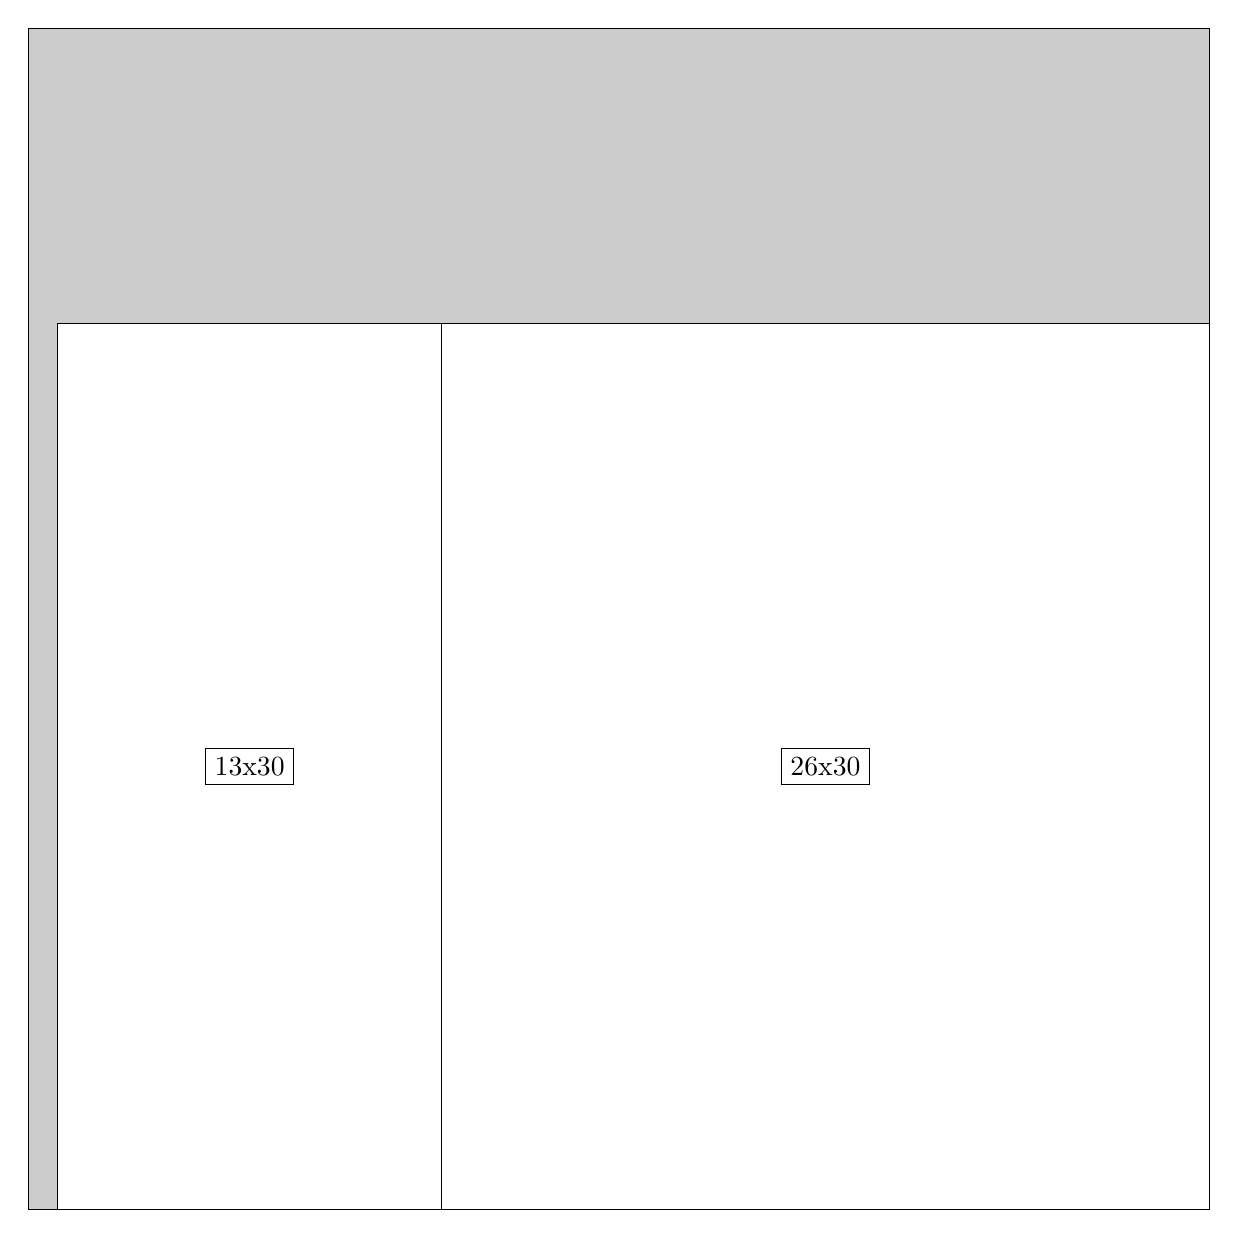
\begin{tikzpicture}[shorten >=1pt,scale=1.0,every node/.style={scale=1.0},->]
\tikzstyle{vertex}=[circle,fill=black!25,minimum size=14pt,inner sep=0pt]
\filldraw[fill=gray!40!white, draw=black] (0,0) rectangle (15.0,15.0);
\foreach \name/\x/\y/\w/\h in {26x30/5.25/0.0/9.75/11.25,13x30/0.375/0.0/4.875/11.25}
\filldraw[fill=white!40!white, draw=black] (\x,\y) rectangle node[draw] (\name) {\name} ++(\w,\h);
\end{tikzpicture}


w =26 , h =30 , x =14 , y =0 , v =780
\par
w =13 , h =30 , x =1 , y =0 , v =390
\par
\newpage


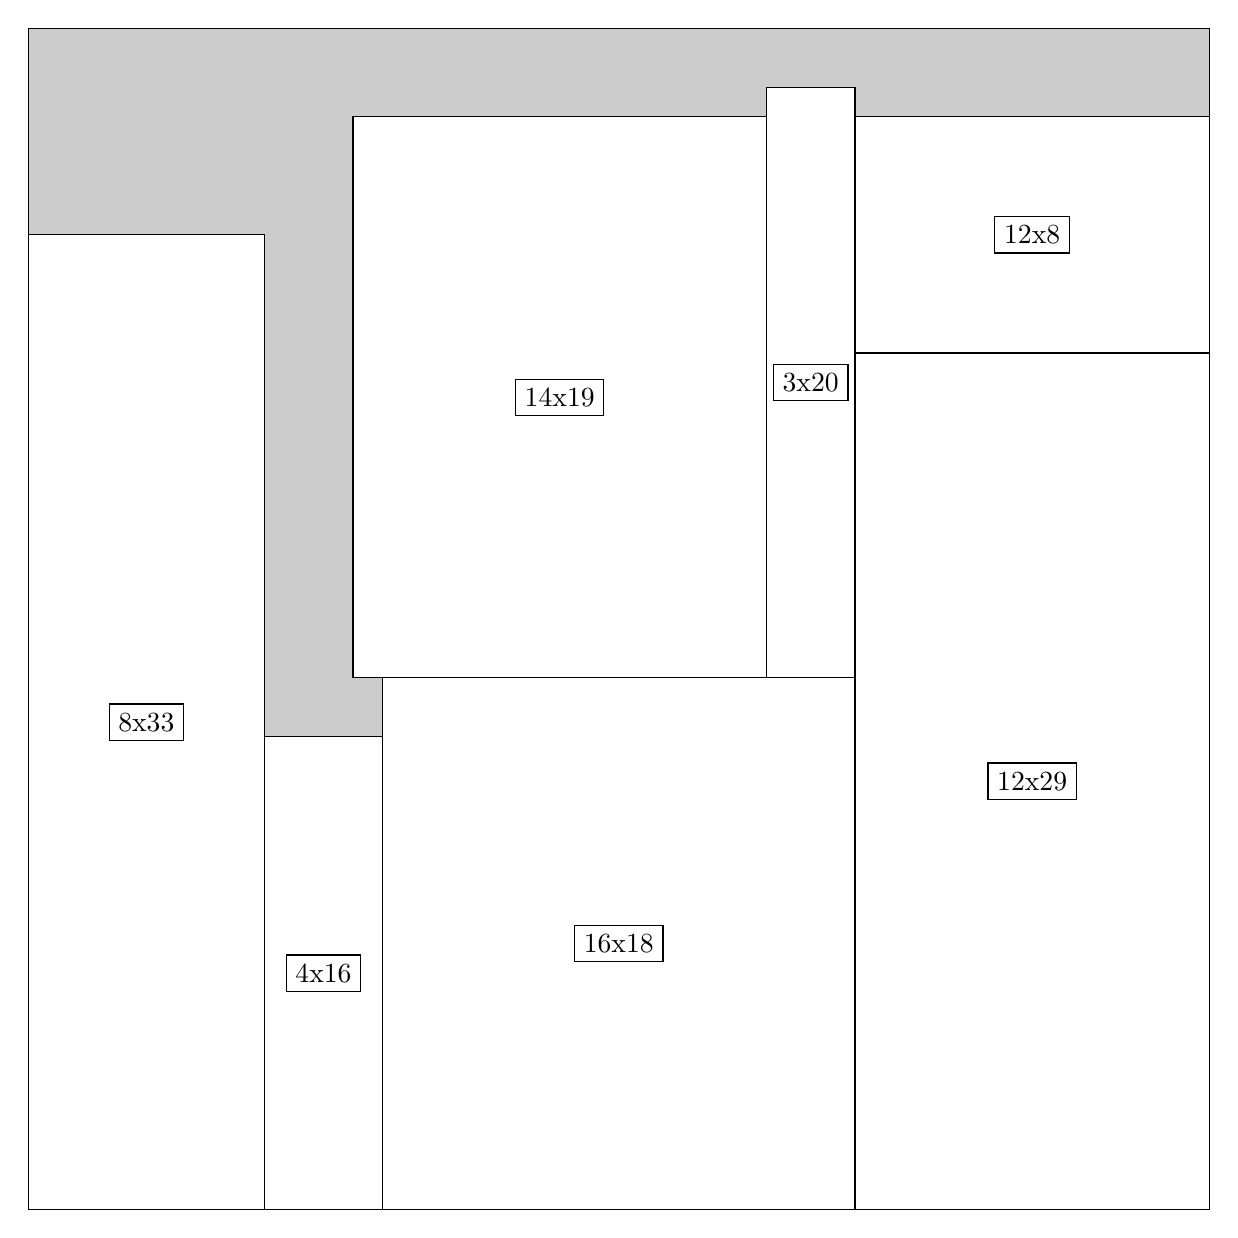
\begin{tikzpicture}[shorten >=1pt,scale=1.0,every node/.style={scale=1.0},->]
\tikzstyle{vertex}=[circle,fill=black!25,minimum size=14pt,inner sep=0pt]
\filldraw[fill=gray!40!white, draw=black] (0,0) rectangle (15.0,15.0);
\foreach \name/\x/\y/\w/\h in {12x29/10.5/0.0/4.5/10.875,12x8/10.5/10.875/4.5/3.0,16x18/4.5/0.0/6.0/6.75,4x16/3.0/0.0/1.5/6.0,3x20/9.375/6.75/1.125/7.5,14x19/4.125/6.75/5.25/7.125,8x33/0.0/0.0/3.0/12.375}
\filldraw[fill=white!40!white, draw=black] (\x,\y) rectangle node[draw] (\name) {\name} ++(\w,\h);
\end{tikzpicture}


w =12 , h =29 , x =28 , y =0 , v =348
\par
w =12 , h =8 , x =28 , y =29 , v =96
\par
w =16 , h =18 , x =12 , y =0 , v =288
\par
w =4 , h =16 , x =8 , y =0 , v =64
\par
w =3 , h =20 , x =25 , y =18 , v =60
\par
w =14 , h =19 , x =11 , y =18 , v =266
\par
w =8 , h =33 , x =0 , y =0 , v =264
\par
\newpage


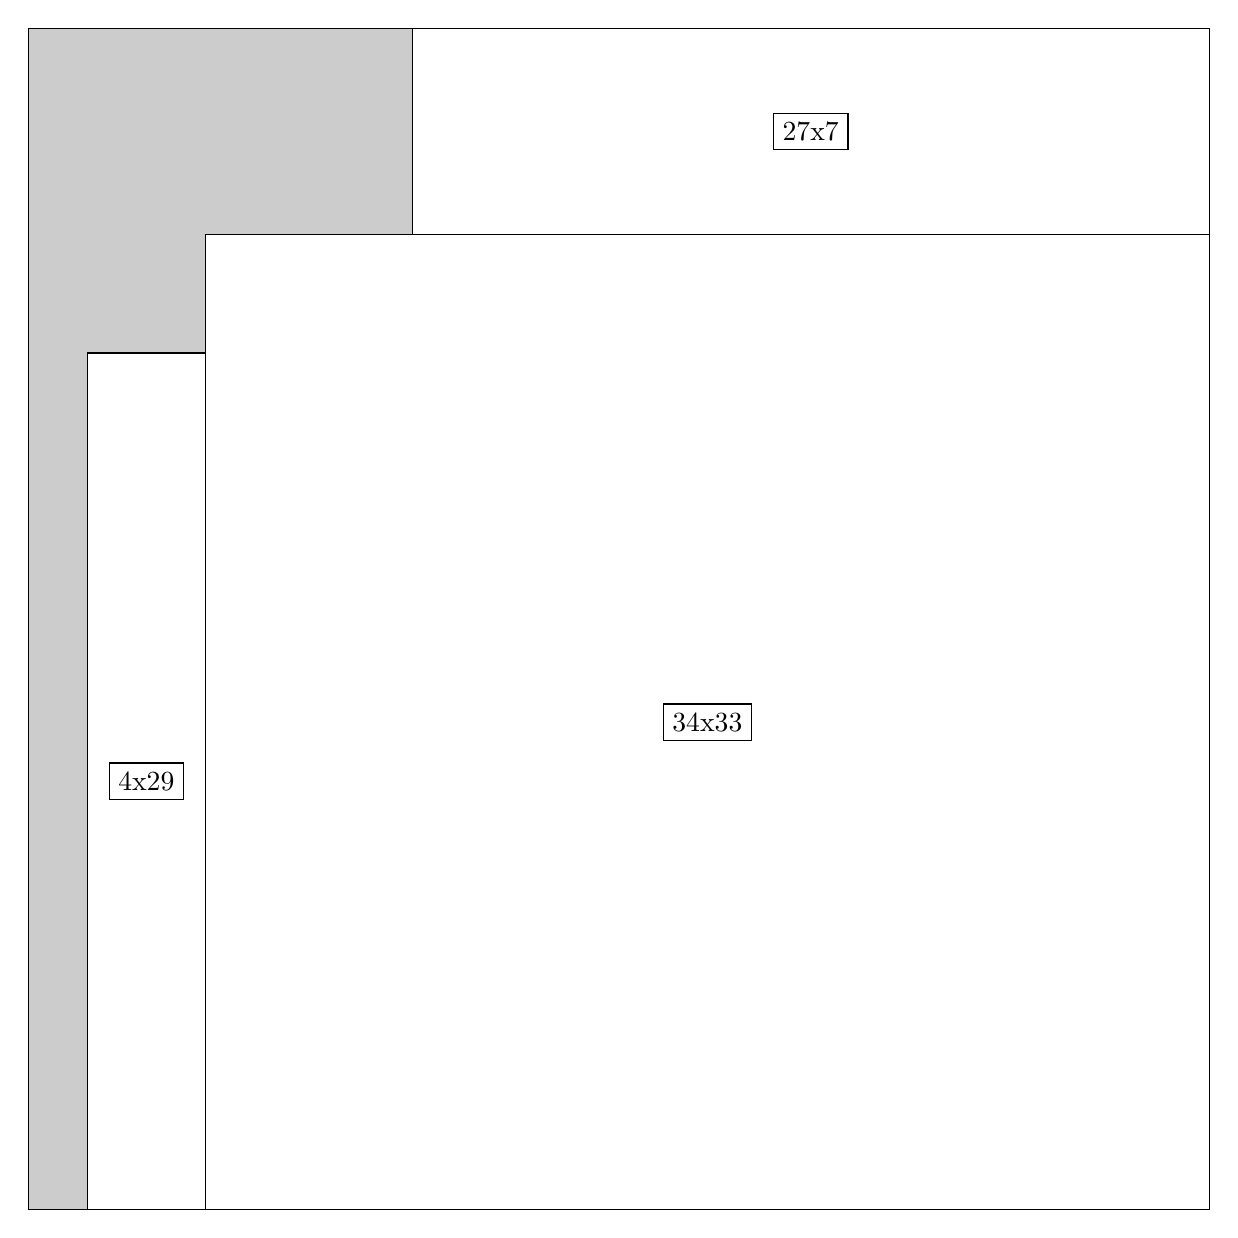
\begin{tikzpicture}[shorten >=1pt,scale=1.0,every node/.style={scale=1.0},->]
\tikzstyle{vertex}=[circle,fill=black!25,minimum size=14pt,inner sep=0pt]
\filldraw[fill=gray!40!white, draw=black] (0,0) rectangle (15.0,15.0);
\foreach \name/\x/\y/\w/\h in {34x33/2.25/0.0/12.75/12.375,27x7/4.875/12.375/10.125/2.625,4x29/0.75/0.0/1.5/10.875}
\filldraw[fill=white!40!white, draw=black] (\x,\y) rectangle node[draw] (\name) {\name} ++(\w,\h);
\end{tikzpicture}


w =34 , h =33 , x =6 , y =0 , v =1122
\par
w =27 , h =7 , x =13 , y =33 , v =189
\par
w =4 , h =29 , x =2 , y =0 , v =116
\par
\newpage


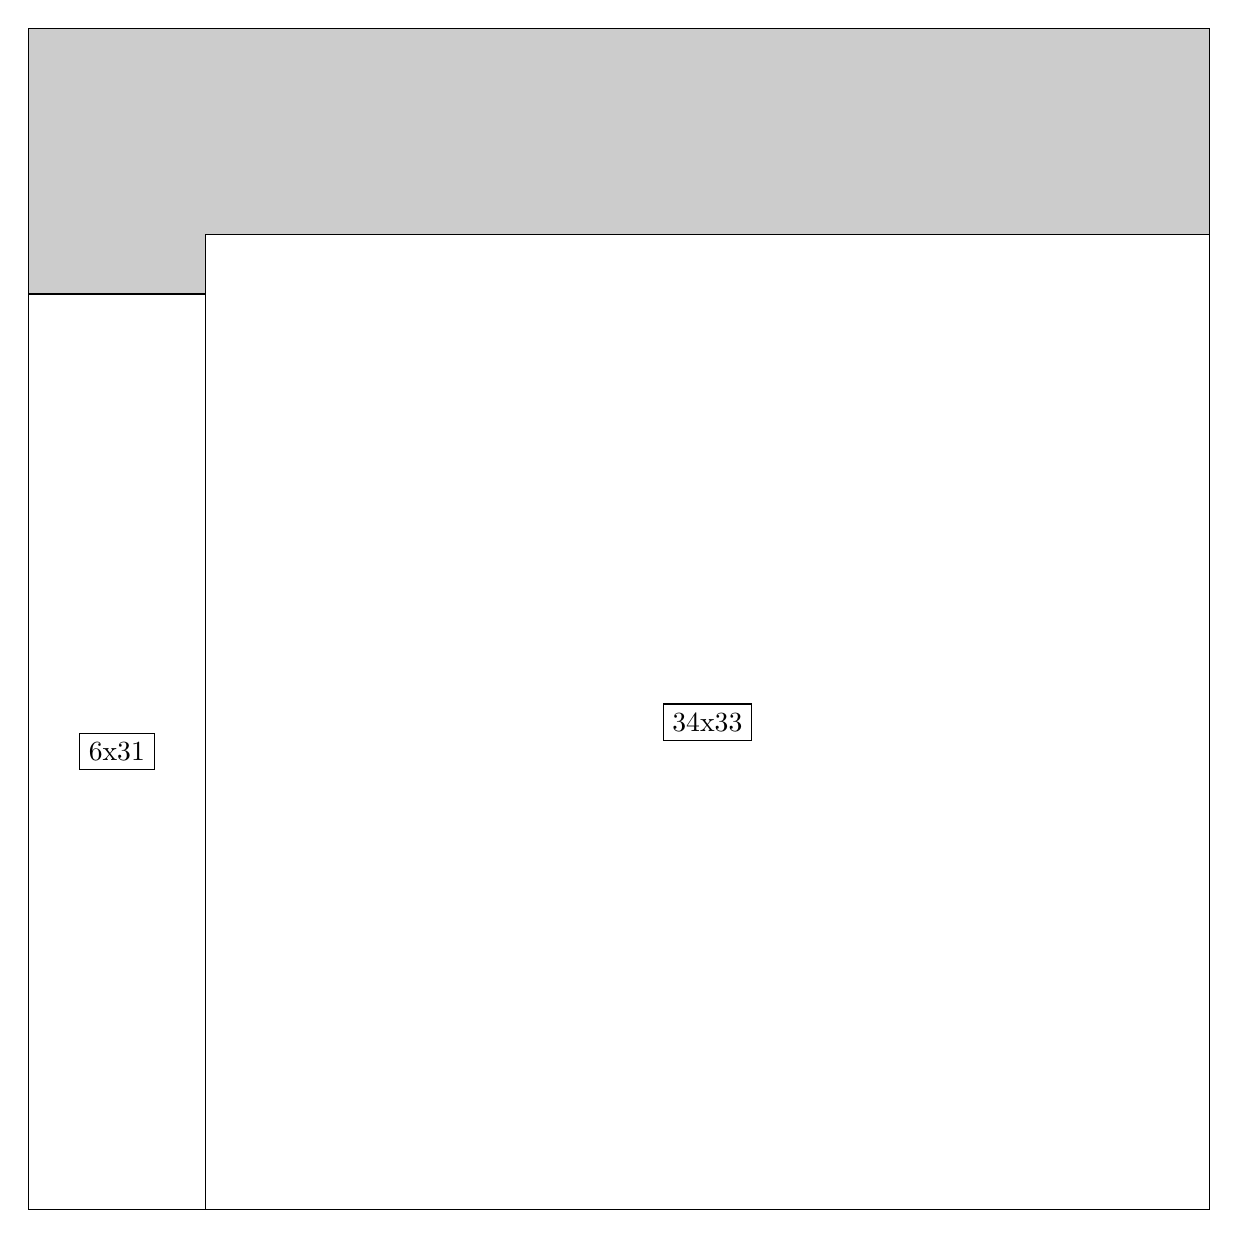
\begin{tikzpicture}[shorten >=1pt,scale=1.0,every node/.style={scale=1.0},->]
\tikzstyle{vertex}=[circle,fill=black!25,minimum size=14pt,inner sep=0pt]
\filldraw[fill=gray!40!white, draw=black] (0,0) rectangle (15.0,15.0);
\foreach \name/\x/\y/\w/\h in {34x33/2.25/0.0/12.75/12.375,6x31/0.0/0.0/2.25/11.625}
\filldraw[fill=white!40!white, draw=black] (\x,\y) rectangle node[draw] (\name) {\name} ++(\w,\h);
\end{tikzpicture}


w =34 , h =33 , x =6 , y =0 , v =1122
\par
w =6 , h =31 , x =0 , y =0 , v =186
\par
\newpage


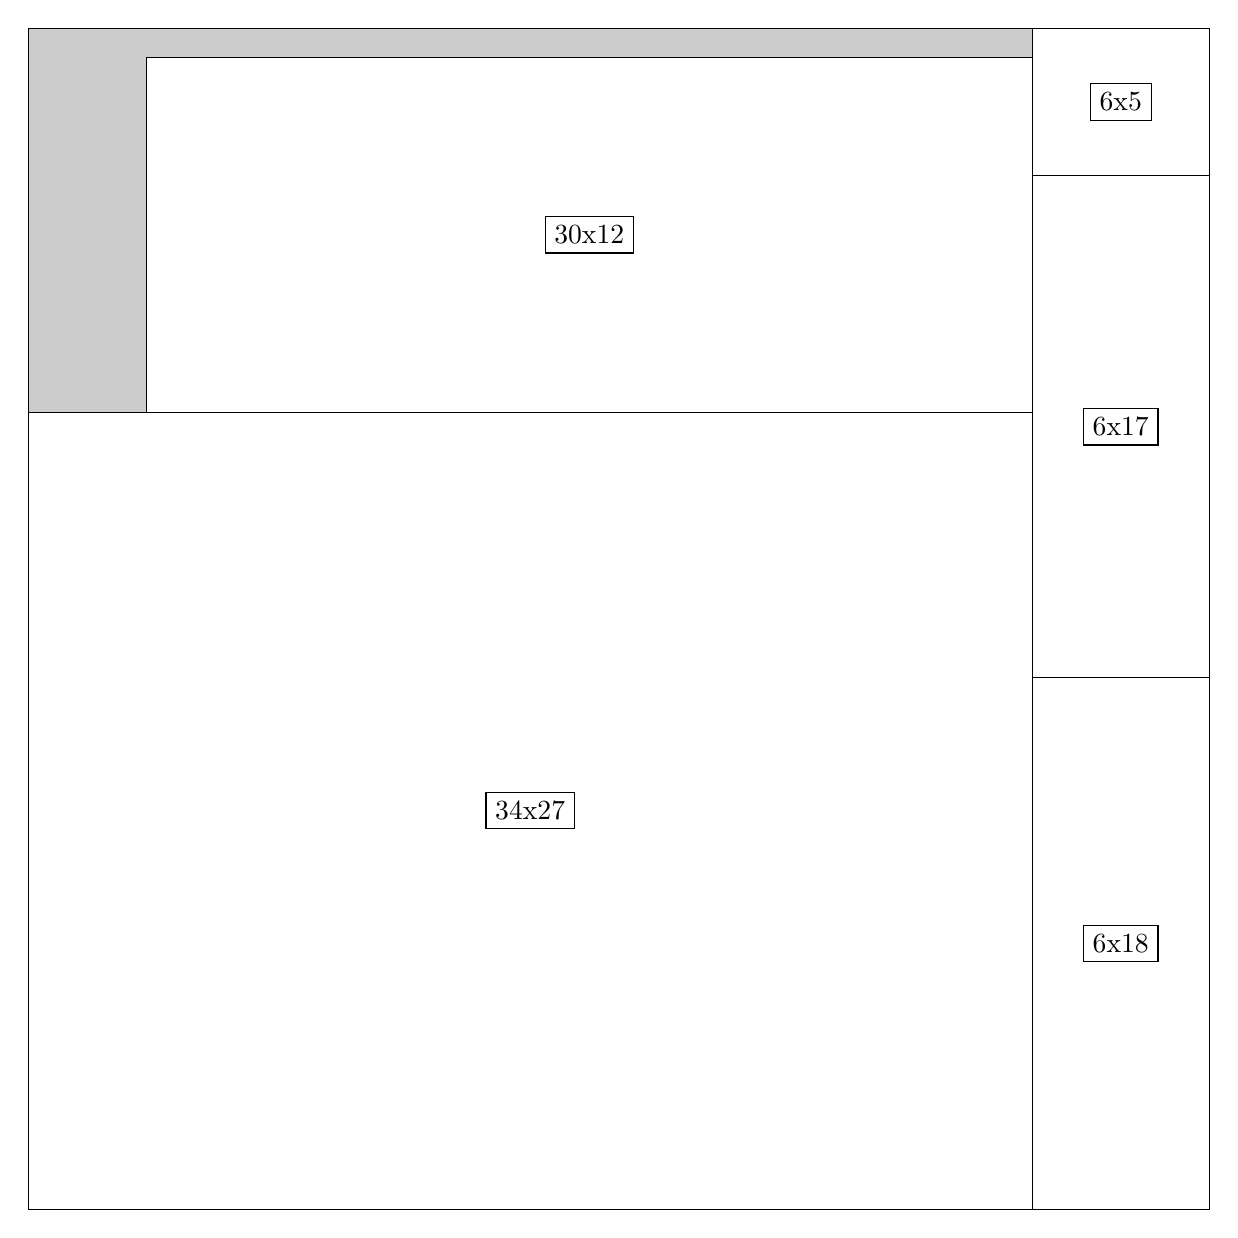
\begin{tikzpicture}[shorten >=1pt,scale=1.0,every node/.style={scale=1.0},->]
\tikzstyle{vertex}=[circle,fill=black!25,minimum size=14pt,inner sep=0pt]
\filldraw[fill=gray!40!white, draw=black] (0,0) rectangle (15.0,15.0);
\foreach \name/\x/\y/\w/\h in {6x18/12.75/0.0/2.25/6.75,6x17/12.75/6.75/2.25/6.375,6x5/12.75/13.125/2.25/1.875,34x27/0.0/0.0/12.75/10.125,30x12/1.5/10.125/11.25/4.5}
\filldraw[fill=white!40!white, draw=black] (\x,\y) rectangle node[draw] (\name) {\name} ++(\w,\h);
\end{tikzpicture}


w =6 , h =18 , x =34 , y =0 , v =108
\par
w =6 , h =17 , x =34 , y =18 , v =102
\par
w =6 , h =5 , x =34 , y =35 , v =30
\par
w =34 , h =27 , x =0 , y =0 , v =918
\par
w =30 , h =12 , x =4 , y =27 , v =360
\par
\newpage


\end{document}